\documentclass[14pt,a4paper]{article}
\usepackage{mathtools}
\usepackage{amsmath}
\setcounter{MaxMatrixCols}{20}
\usepackage{bigints}
\usepackage{mathrsfs}
\usepackage{setspace}
\usepackage{amsfonts}
\usepackage{geometry}
\geometry{a4paper, total = {210mm,297mm},left=35mm, right=25mm,top=25mm,bottom=25mm}
\usepackage{xcolor}
\usepackage{mcode}
\usepackage{listings}
\lstset{basicstyle = \fontsize{11}{12} \selectfont\ttfamily}
\usepackage{graphicx}


%Begin document - Numerical Analysis - Homework 2

\begin{document}
\label{cover}
\begin{center}
	\vspace*{3cm}
	\large{\textbf{MATH/CS 5466 NUMERICAL ANALYSIS \\ Homework 2}}
	\vfill
	\textbf{Luan Cong Doan} \\ luandoan@vt.edu
	%\vfill
%	Department of Mechanical Engineering \\ Virginia Polytechnic Institute and State University
	\vfill
	\today
\end{center}
\pagebreak

\label{Answer Sheet - Numerical Homework 2}
\doublespacing
Several of the problems use the \textit{infinity form} of a function $g \in [a,b]$, defined by:\\
\hspace*{5cm} $\|g\|_{\infty} = \max\limits_{a\leq x \leq b}|g(x)|$ \\
This norm defines the usual norm axiom:\\
(i) $\|g\|_{\infty} \geq 0$ for all $g \in [a,b]$ and $\|g\|_{\infty} = 0$ if and only if $g(x) = 0$ for all $x \in [a,b]$\\
(ii) $\|\alpha g\|_{\infty} = |\alpha|\|g\|_{\infty}$ for all $g \in [a,b]$ and all $\alpha \in \mathbb{R}$; \\
(iii) $\|g+h\|_{\infty} \leq \|g\|_{\infty} + \|h\|_{\infty}$ for all $g,h \in C[a,b]$.\\

\label{Problem 1}
\large\textbf{Problem 1.} The construction of finite difference approximations of differential equations, developing a second order accurate approximation of the boundary value problem$-u"(x) = g(x)$ for $x \in [0,1]$ with $u(0) = u(1) = 0$.\\
With the uniformly space grid:\\
\hspace*{3cm} $ 0 = x_0 < x_1 < ... < x_{n-1} < x_n = 1$ \hspace{0.5cm} 
with $x_j = jh$ for $h = 1/n$.

\begin{enumerate}
	\label{1a}
	\item Compute the \textit{quartic} (degree 4) polynomial interpolant $p_4$ to a function $f(x)$ through the five points: $x_{j-2}, x_{j-1}, x_j, x_{j+1}, x_{j+2}$\\
	with the five function values $f_{-2}  \equiv f(x_{j-2}), f_{-1} \equiv f(x_{j-1}), f_0 \equiv f(x_j), f_1 \equiv f(x_{j+1}), f_2 \equiv f(x_{j+2})$: \\
	Base on \textit{Lagrange Interpolation Formula}:
	$$ p_n(x) = \sum_{i=0}^nf_il_i(x) \hspace{2cm} with \hspace{0.5cm} l_i(x) = \prod_{j=0,j \neq i}^{n} \dfrac{x-x_j}{x_i-x_j}$$
	for $n =4$ over $5$ given points we have:\\
	\hspace*{1cm}$p_4(x) = f_{-2}l_{-2}(x) + f_{-1}l_{-1}(x) + f_0l_0(x) + f_1l_1(x) + f_2l_2(x)$\\
	With: \hspace{0.5cm} $l_{-2}(x) = \dfrac{(x-x_{j-1})(x-x_j)(x-x_{j+1})(x-x_{j+2})}{(x_{j-2}-x_{j-1})(x_{j-2}-x_j)(x_{j-2}-x_{j+1})(x_{j-2}-x_{j+2})} $\\
	\hspace*{2.95cm} $= \dfrac{(x-x_j +h)(x-x_j)(x-x_j-h)(x-x_j-2h)}{(-h)(-2h)(-3h)(-4h)}$\\
	\hspace*{2.95cm} $= \dfrac{[(x-x_j)^2 -h^2][(x-x_j)^2 -2h(x-x_j)]}{24h^4} $\\
	\hspace*{2.95cm} $= \dfrac{(x^2 - 2xx_j + x_j^2 -h^2)(x^2 - 2(x_j+h)x +x_j^2 +2hx_j)}{24h^4}$\\
	\hspace*{2.95cm}	$= \dfrac{x^4 - (4x_j+2h)x^3 +(6x_j^2 + 6hx_j -h^2)x^2 }{24h^4} \\
	\hspace*{3.5cm} + \dfrac{- (4x_j^3 +6hx_j^2 -2h^2x_j -2h^3)x + (x_j^2-h^2)(x_j^2+2hx_j)}{24h^4}$\\
	
	%$= \dfrac{x^4 - (4x_j+2h)x^3 +(6x_j^2 + 6hx_j -h^2)x^2 - (6x_j^3 +6hx_j^2 -2h^2x_j -2h^3)x + (x_j^2-h^2)(x_j^2+2hx_j)}{24h^4}$\\
	
	
	$l_{-1}(x) = \dfrac{(x-x_{j-2})(x-x_j)(x-x_{j+1})(x-x_{j+2})}{(x_{j-1}-x_{j-2})(x_{j-1}-x_j)(x_{j-1}-x_{j+1})(x_{j-1}-x_{j+2})} $\\
	\hspace*{1.1cm} $= \dfrac{(x-x_j +2h)(x-x_j)(x-x_j-h)(x-x_j-2h)}{(h)(-h)(-2h)(-3h)}$\\
	\hspace*{1.1cm} $= -\dfrac{[(x-x_j)^2 -4h^2][(x-x_j)^2 -h(x-x_j)]}{6h^4} $\\
	\hspace*{1.1cm} $= -\dfrac{(x^2 - 2xx_j + x_j^2 -4h^2)(x^2 - (2x_j+h)x +x_j^2 +hx_j)}{6h^4}$\\
	\hspace*{1.1cm} $= -\dfrac{x^4 -(4x_j+h)x^3 +(6x_j^2 +3hx_j-4h^2)x^2}{6h^4}$\\
	\hspace*{1.7cm} $- \dfrac{-(4x_j^3 +3hx_j^2-8h^2x_j-4h^3)x +(x_j^2-4h^2)(x_j^2+hx_j)}{6h^4}$\\
	
	
	$l_0(x) = \dfrac{(x-x_{j-2})(x-x_{j-1})(x-x_{j+1})(x-x_{j+2})}{(x_j-x_{j-2})(x_j-x_{j-1})(x_j-x_{j+1})(x_j-x_{j+2})} $\\
	\hspace*{0.8cm} $= \dfrac{(x-x_j +2h)(x-x_j+h)(x-x_j-h)(x-x_j-2h)}{(2h)(h)(-h)(-2h)}$\\
	\hspace*{0.8cm} $= \dfrac{[(x-x_j)^2 -4h^2][(x-x_j)^2 -h^2]}{4h^4} $\\
	\hspace*{0.8cm} $= \dfrac{(x^2 - 2xx_j + x_j^2 -4h^2)(x^2 - 2xx_j +x_j^2 -h^2)}{4h^4}$\\
	\hspace*{0.8cm} $= \dfrac{x^4 -4x_jx^3 +(6x_j^2-5h^2)x^2 -(4x_j^3-10h^2x_j)x +(x_j^2-4h^2)(x_j^2-h^2)}{4h^4}$\\
	
	$l_1(x) = \dfrac{(x-x_{j-2})(x-x_{j-1})(x-x_j)(x-x_{j+2})}{(x_{j+1}-x_{j-2})(x_{j+1}-x_{j-1})(x_{j+1}-x_j)(x_{j+1}-x_{j+2})} $\\
	\hspace*{0.8cm} $= \dfrac{(x-x_j +2h)(x-x_j+h)(x-x_j)(x-x_j-2h)}{(3h)(2h)(h)(-h)}$\\
	\hspace*{0.8cm} $= -\dfrac{[(x-x_j)^2 -4h^2][(x-x_j)^2 +h(x-x_j)]}{6h^4} $\\
	\hspace*{0.8cm} $= \dfrac{(x^2 - 2xx_j + x_j^2 -4h^2)(x^2 - (2x_j-h)x +x_j^2 -hx_j)}{4h^4}$\\
	\hspace*{0.8cm}$ = -\dfrac{x^4 -(4x_j-h)x^3 +(6x_j^2 -3hx_j-4h^2)x^2}{6h^4}$\\
	\hspace*{1.7cm} $- \dfrac{-(4x_j^3 -3hx_j^2-8h^2x_j+4h^3)x +(x_j^2-4h^2)(x_j^2-hx_j)}{6h^4}$\\
	
	$l_2(x) = \dfrac{(x-x_{j-2})(x-x_{j-1})(x-x_j)(x-x_{j+1})}{(x_{j+2}-x_{j-2})(x_{j+2}-x_{j-1})(x_{j+2}-x_j)(x_{j+2}-x_{j+1})} $\\
	\hspace*{0.8cm} $= \dfrac{(x-x_j +2h)(x-x_j+h)(x-x_j)(x-x_j-h)}{(4h)(3h)(2h)(h)}$\\
	\hspace*{0.8cm} $= \dfrac{[(x-x_j)^2 -h^2][(x-x_j)^2 +2h(x-x_j)]}{24h^4} $\\
	\hspace*{0.8cm} $= \dfrac{(x^2 - 2xx_j + x_j^2 -h^2)(x^2 - 2(x_j-h)x +x_j^2 -2hx_j)}{24h^4}$\\
	\hspace*{0.8cm}	$= \dfrac{x^4 - (4x_j-2h)x^3 +(6x_j^2 - 6hx_j -h^2)x^2 }{24h^4} \\
	\hspace*{1.7cm} + \dfrac{- (4x_j^3 -6hx_j^2 -2h^2x_j +2h^3)x + (x_j^2-h^2)(x_j^2+2hx_j)}{24h^4}$
	\pagebreak
	
	\label{1b}
	\item Compute $p''_4(x_j)$ and simplify as much as possible:\\
	because $f_{-2}, f_{-1},f_0,f_1,f_2$ are all constants so: \\
	\hspace*{3cm} $p''_4(x) = f_{-2}.l''_{-2} + f_{-1}l''_{-1} + f_0l''_0 +f_1l''_1 + f_2l''_2$\\
	Base on computed $l_{-2}, l_{-1},l_0,l_1,l_2$ above, we have:\\
	$\bullet$ $ l'_{-2}(x) = \dfrac{4x^3- 3(4x_j+2h)x^2 + 2(6x_j^2+6hx_j-h^2)x -(4x_j^3+6hx_j^2-2h^2x_j -2h^3)}{24h^4}$\\
	\hspace*{0.2cm} $l''_{-2}(x) = \dfrac{12x^2 - 6(4x_j+2h)x+2(6x_j^2+6hx_j-h^2)}{24h^4}$\\
	\hspace*{0.2cm} $l''_{-2}(x_j) = \dfrac{1}{24h^4} (12x_j^2 -6(4x_j+2h)x_j + 12x_j^2 + 12hx_j -2h^2)$\\
	\hspace*{1.6cm} $ = -\dfrac{1}{12h^2}$\\
	
	$\bullet$ $ l'_{-1}(x) = - \dfrac{4x^3 -3(4x_j+h)x^2 + 2(6x_j^2 +3hx_j -4h^2)x -(4x_j^3 +3hx_j^2 -8h^2x_j -4h^3)}{6h^4} $\\
	\hspace*{0.2cm} $l''_{-1}(x) = - \dfrac{12x^2 -6(4x_j+h)x +2(6x_j^2 + 3hx_j -4h^2)}{6h^4}$\\
	\hspace*{0.2cm} $l''_{-1}(x_j) = -\dfrac{1}{6h^4} [12x_j^2 -6(4x_j+h)x_j + 12x_j^2 +6hx_j -8h^2]$\\
	\hspace*{1.6cm} $ = \dfrac{4}{3h^2}$\\
	
	$\bullet$ $ l'_0(x) = \dfrac{4x^3 -12x_jx^2 + 2(6x_j^2 -5h^2)x -(4x_j^3-10h^2x_j)}{4h^4}$\\
	\hspace*{0.2cm} $l''_0(x) = \dfrac{12x^2 - 24x_jx + 12x_j^2 -10h^2}{4h^4}$\\
	\hspace*{0.2cm} $l''_0(x_j) = \dfrac{1}{4h^4} (12x_j^2 - 24x_j.x_j + 12x_j^2 -10h^2)$\\
	\hspace*{1.4cm} $ = - \dfrac{5}{2h^2}$\\
	
	$\bullet$ $ l'_1(x) = - \dfrac{4x^3 -3(4x_j-h)x^2 + 2(6x_j^2 -3hx_j -4h^2)x -(4x_j^3 -3hx_j^2 -8h^2x_j +4h^3)}{6h^4} $\\
	\hspace*{0.2cm} $l''_1(x) = - \dfrac{12x^2 -6(4x_j-h)x +2(6x_j^2 - 3hx_j -4h^2)}{6h^4}$\\
	\hspace*{0.2cm} $l''_1(x_j) = -\dfrac{1}{6h^4} [12x_j^2 -6(4x_j-h)x_j + 12x_j^2 -6hx_j -8h^2]$\\
	\hspace*{1.4cm} $ = \dfrac{4}{3h^2}$\\
	
	$\bullet$ $ l'_2(x) = \dfrac{4x^3- 3(4x_j-2h)x^2 + 2(6x_j^2+6hx_j-h^2)x -(4x_j^3-6hx_j^2-2h^2x_j +2h^3)}{24h^4}$\\
	\hspace*{0.2cm} $l''_2(x) = \dfrac{12x^2 - 6(4x_j-2h)x+2(6x_j^2-6hx_j-h^2)}{24h^4}$\\
	\hspace*{0.2cm} $l''_2(x_j) = \dfrac{1}{24h^4} (12x_j^2 -6(4x_j-2h)x_j + 12x_j^2 - 12hx_j -2h^2)$\\
	\hspace*{1.4cm} $ = -\dfrac{1}{12h^2}$
	\pagebreak
	
	So: \hspace{0.3cm} $p''_4(x_j) = f_{-2}.\dfrac{-1}{12h^2} + f_{-1}.\dfrac{4}{3h^2} +f_0.\dfrac{-5}{2h^2} + f_1.\dfrac{4}{3h^2} + f_2.\dfrac{-1}{12h^2} $\\
	\hspace*{2.4cm} $ = \dfrac{-\dfrac{1}{12}f_{-2} + \dfrac{4}{3}f_{-1} - \dfrac{5}{2}f_0 + \dfrac{4}{3}f_1 - \dfrac{1}{12}f_2}{h^2} $\\
	three constants are defined as follow: $ A = -\dfrac{1}{12}; \hspace{0.3cm} B = \dfrac{4}{3}; \hspace{0.3cm} C = -\dfrac{5}{2}$\\
	
	\label{1c}
	\item Compute $p"_4(x_{j-1})$ and $p"_4(x_{j+1})$:\\
	Based on above analyzing we have: $x_{j-1} = x_j -h, x_{j+1} = x_j+h$ and: \\
	$l''_{-2}(x_{j-1}) = \dfrac{1}{24h^4} [12x_{j-1}^2 -6(4x_j+2h)x_{j-1} + 12x_j^2 + 12hx_j -2h^2]$\\
	\hspace*{1.6cm} $ = \dfrac{1}{24h^4}[12(x_j-h)^2 -6(4x_j+2h)(x_j-h) +12x_j^2 + 12hx_j -2h^2] $\\
	\hspace*{1.6cm} $ = \dfrac{1}{24h^4}[12x_j^2 -24hx_j +12h^2 -24x_j^2 +12hx_j + 12h^2 + 12x_j^2 + 12hx_j -2h^2] $\\
	\hspace*{1.6cm} $ = \dfrac{11}{12h^2}$\\
	
	$l''_{-2}(x_{j+1}) = \dfrac{1}{24h^4} [12x_{j+1}^2 -6(4x_j+2h)x_{j+1} + 12x_j^2 + 12hx_j -2h^2]$\\
	\hspace*{1.6cm} $ = \dfrac{1}{24h^4}[12(x_j+h)^2 -6(4x_j+2h)(x_j+h) +12x_j^2 + 12hx_j -2h^2] $\\
	\hspace*{1.6cm} $ = \dfrac{1}{24h^4}[12x_j^2 +24hx_j +12h^2 -24x_j^2 -36hx_j - 12h^2 + 12x_j^2 + 12hx_j -2h^2] $\\
	\hspace*{1.6cm} $ = -\dfrac{1}{12h^2}$\\
	
	$l''_{-1}(x_{j-1}) = -\dfrac{1}{6h^4} [12x_{j-1}^2 -6(4x_j+h)x_{j-1} + 12x_j^2 +6hx_j -8h^2]$\\
	\hspace*{1.6cm} $ = -\dfrac{1}{6h^4} [12(x_j-h)^2 -6(4x_j+h)(x_j-h) + 12x_j^2 +6hx_j -8h^2]$\\
	\hspace*{1.6cm} $ = -\dfrac{1}{6h^4} [12x_j^2 -24hx_j +12h^2 -24x_j^2 +18hx_j +6h^2 + 12x_j^2 +6hx_j -8h^2]$\\
	\hspace*{1.6cm} $ = -\dfrac{5}{3h^2}$\\
	
	$l''_{-1}(x_{j+1}) = -\dfrac{1}{6h^4} [12x_{j+1}^2 -6(4x_j+h)x_{j+1} + 12x_j^2 +6hx_j -8h^2]$\\
	\hspace*{1.6cm} $ = -\dfrac{1}{6h^4} [12(x_j+h)^2 -6(4x_j+h)(x_j+h) + 12x_j^2 +6hx_j -8h^2]$\\
	\hspace*{1.6cm} $ = -\dfrac{1}{6h^4} [12x_j^2 +24hx_j +12h^2 -24x_j^2 -30hx_j -6h^2 + 12x_j^2 +6hx_j -8h^2]$\\
	\hspace*{1.6cm} $ = \dfrac{1}{3h^2}$\\
	
	$l''_0(x_{j-1}) = \dfrac{1}{4h^4} (12x_{j-1}^2 - 24x_j.x_{j-1} + 12x_j^2 -10h^2)$\\
	\hspace*{1.4cm} $ = \dfrac{1}{4h^4} (12(x_j-h)^2 - 24x_j(x_j-h) + 12x_j^2 -10h^2)$\\
	\hspace*{1.4cm} $ = \dfrac{1}{4h^4} (12x_j^2 -24hx_j +12h^2 - 24x_j^2 +24hx_j + 12x_j^2 -10h^2)$\\
	\hspace*{1.4cm} $ = \dfrac{1}{2h^2}$\\
	
	$l''_0(x_{j+1}) = \dfrac{1}{4h^4} (12x_{j+1}^2 - 24x_j.x_{j+1} + 12x_j^2 -10h^2)$\\
	\hspace*{1.4cm} $ = \dfrac{1}{4h^4} (12(x_j+h)^2 - 24x_j(x_j+h) + 12x_j^2 -10h^2)$\\
	\hspace*{1.4cm} $ = \dfrac{1}{4h^4} (12x_j^2 +24hx_j +12h^2 - 24x_j^2 -24hx_j + 12x_j^2 -10h^2)$\\
	\hspace*{1.4cm} $ = \dfrac{1}{2h^2}$\\
	
	$l''_1(x_{j-1}) = -\dfrac{1}{6h^4} [12x_{j-1}^2 -6(4x_j-h)x_{j-1} + 12x_j^2 -6hx_j -8h^2]$\\
	\hspace*{1.4cm} $ = -\dfrac{1}{6h^4} [12(x_j-h)^2 -6(4x_j-h)(x_j-h) + 12x_j^2 -6hx_j -8h^2]$\\
	\hspace*{1.4cm} $ = -\dfrac{1}{6h^4} [12x_j^2 -24hx_j +12h^2 -24x_j^2 +30hx_j -6h^2 + 12x_j^2 -6hx_j -8h^2]$\\
	\hspace*{1.4cm} $ = \dfrac{1}{3h^2}$\\
	
	$l''_1(x_{j+1}) = -\dfrac{1}{6h^4} [12x_{j+1}^2 -6(4x_j-h)x_{j+1} + 12x_j^2 -6hx_j -8h^2]$\\
	\hspace*{1.4cm} $ = -\dfrac{1}{6h^4} [12(x_j+h)^2 -6(4x_j-h)(x_j+h) + 12x_j^2 -6hx_j -8h^2]$\\
	\hspace*{1.4cm} $ = -\dfrac{1}{6h^4} [12x_j^2 +24hx_j +12h^2 -24x_j^2 -18hx_j +6h^2 + 12x_j^2 -6hx_j -8h^2]$\\
	\hspace*{1.4cm} $ = -\dfrac{5}{3h^2}$\\
	
	$l''_2(x_{j-1}) = \dfrac{1}{24h^4} (12x_{j-1}^2 -6(4x_j-2h)x_{j-1} + 12x_j^2 - 12hx_j -2h^2)$\\
	\hspace*{1.4cm} $ = \dfrac{1}{24h^4} (12(x_j-h)^2 -6(4x_j-2h)(x_j-h) + 12x_j^2 - 12hx_j -2h^2)$\\
	\hspace*{1.4cm} $ = \dfrac{1}{24h^4} (12x_j^2 -24hx_j +12h^2 -24x_j^2 +36hx_j -12h^2 + 12x_j^2 - 12hx_j -2h^2)$\\
	\hspace*{1.4cm} $ = -\dfrac{1}{12h^2}$\\
	
	$l''_2(x_{j+1}) = \dfrac{1}{24h^4} (12x_{j+1}^2 -6(4x_j-2h)x_{j+1} + 12x_j^2 - 12hx_j -2h^2)$\\
	\hspace*{1.4cm} $ = \dfrac{1}{24h^4} (12(x_j+h)^2 -6(4x_j-2h)(x_j+h) + 12x_j^2 - 12hx_j -2h^2)$\\
	\hspace*{1.4cm} $ = \dfrac{1}{24h^4} (12x_j^2 +24hx_j +12h^2 -24x_j^2 -12hx_j +12h^2 + 12x_j^2 - 12hx_j -2h^2)$\\
	\hspace*{1.4cm} $ = \dfrac{11}{12h^2}$
	\pagebreak
	
	So: \hspace{0.3cm} $p''_4(x_{j-1}) = f_{-2}.\dfrac{11}{12h^2} + f_{-1}.\dfrac{-5}{3h^2} +f_0.\dfrac{1}{2h^2} + f_1.\dfrac{1}{3h^2} + f_2.\dfrac{-1}{12h^2} $\\
	\hspace*{2.7cm} $ = \dfrac{\dfrac{11}{12}f_{-2} - \dfrac{5}{3}f_{-1} + \dfrac{1}{2}f_0 + \dfrac{1}{3}f_1 - \dfrac{1}{12}f_2}{h^2} $\\
	
	\hspace*{1cm} $p''_4(x_{j+1}) = f_{-2}.\dfrac{-1}{12h^2} + f_{-1}.\dfrac{1}{3h^2} +f_0.\dfrac{1}{2h^2} + f_1.\dfrac{-5}{3h^2} + f_2.\dfrac{11}{12h^2} $\\
	\hspace*{2.7cm} $ = \dfrac{-\dfrac{1}{12}f_{-2} + \dfrac{1}{3}f_{-1} + \dfrac{1}{2}f_0 - \dfrac{5}{3}f_1 + \dfrac{11}{12}f_2}{h^2} $\\
	
	five constants are: $ D = \dfrac{11}{12}; \hspace{0.3cm} E = -\dfrac{5}{3}; \hspace{0.3cm} F = \dfrac{1}{2}; \hspace{0.3cm} G = \dfrac{1}{3}; \hspace{0.3cm} H = -\dfrac{1}{12}$\\
	
	\label{1d}
	\item We are now prepare to approximate the solution to the differential equation: \\
	\hspace*{4cm} $-u"(x) = g(x)$, \hspace{1cm} $u(0) = u(1) = 0$\\
	Construct the quartic interpolant $p_{4,j}$ to $u(x)$ at the points $x_{j-2},x_{j-1},x_j,x_{j+1},x_{j+2}$ as done in part 1a, we have the approximation:\\
	\hspace*{2cm} $-p''_4(x_j) \approx -u''(x_j) = g(x_j) \hspace{1cm} and \hspace{0.5cm} u_j \approx u(x_j)$\\
	As result from 1b, we have:\\
	\hspace*{2.7cm} $p''_4(x_j) = \dfrac{-\dfrac{1}{12}f_{-2} + \dfrac{4}{3}f_{-1} - \dfrac{5}{2}f_0 + \dfrac{4}{3}f_1 - \dfrac{1}{12}f_2}{h^2} $\\
	For $j = 1, ..., n$ we have:\\
	$-p''_4(x_1) = -p''_4(x_{2-1}) =  -\dfrac{11}{12h^2}u_0 + \dfrac{5}{3h^2}u_1 - \dfrac{1}{2h^2}u_2 - \dfrac{1}{3h^2}u_3 + \dfrac{1}{12h^2}u_4\\
	\hspace*{3.8cm} = g(x_{2-1}) = g(x_1)$\\
	$-p''_4(x_2) = \dfrac{1}{12h^2}u_0 - \dfrac{4}{3h^2}u_1 + \dfrac{5}{2h^2}u_2 - \dfrac{4}{3h^2}u_3 + \dfrac{1}{12h^2}u_4 = g(x_2)$\\
	\hspace*{0.5cm}   ... ... ...\\
	$-p''_4(x_{n-2}) = \dfrac{1}{12h^2}u_{n-4} - \dfrac{4}{3h^2}u_{n-3} + \dfrac{5}{2h^2}u_{n-2} - \dfrac{4}{3h^2}u_{n-1} + \dfrac{1}{12h^2}u_n = g(x_{n-2})$\\
	$-p''_4(x_{n-1}) = -p''_4(x_{n-2+1}) \\
	\hspace*{1.9cm} = \dfrac{1}{12h^2}u_{n-4} - \dfrac{1}{3h^2}u_{n-3} - \dfrac{1}{2h^2}u_{n-2} + \dfrac{5}{3h^2}u_{n-1} - \dfrac{11}{12h^2}u_n = g(x_{n-1})$\\
	
	We could form a linear system equation: \hspace{0.3cm} $M.u = g$\\
	$\hspace*{1cm} M = \dfrac{1}{h^2}.\begin{bmatrix} \dfrac{5}{3} & -\dfrac{1}{2} & -\dfrac{1}{3}& \dfrac{1}{12} &0& ... & ... & ... &0&0&0&0&0 \\ -\dfrac{4}{3}  &\dfrac{5}{2} & -\dfrac{4}{3} & \dfrac{1}{12} &0& ... & ... & ... &0&0&0&0&0 \\ \dfrac{1}{12} & -\dfrac{4}{3} &\dfrac{5}{2} & -\dfrac{4}{3} & \dfrac{1}{12} & ... & ... & ... &0&0&0&0&0 \\ ...& & ... & & ... & \ddots & & & & ... & & ...\\  ...& & ... & & ... & & & \ddots  & & ... & & ... \\ 0&0&0&0&0 & ... &...&...& 0& \dfrac{1}{12} & -\dfrac{4}{3} &\dfrac{5}{2} & -\dfrac{4}{3} \\ 0&0&0&0&0 & ... &...&...& 0& \dfrac{1}{12} & -\dfrac{1}{3} &-\dfrac{1}{2} & \dfrac{5}{3} \end{bmatrix}$\\
	
	\label{1e}
	\item Produce a $\mathtt{MATLAB}$ implementation of approximation. For $n = 6$: \\
	\hspace*{2.5cm} $ h = \dfrac{1}{n} = \dfrac{1}{6}$.\\
	 So the 5x5 matrix (M) of linear system is: \\
	\hspace*{1cm} $M = \dfrac{1}{(\frac{1}{6})^2}.\begin{bmatrix} \dfrac{5}{3} &-\dfrac{1}{2} & -\dfrac{1}{3} & \dfrac{1}{12} & 0 \\ -\dfrac{4}{3}  &\dfrac{5}{2} & -\dfrac{4}{3} & \dfrac{1}{12} &0 \\ \dfrac{1}{12} & -\dfrac{4}{3} & \dfrac{5}{2} & -\dfrac{4}{3} & \dfrac{1}{12} \\ 0& \dfrac{1}{12} & -\dfrac{4}{3} & \dfrac{5}{2} & -\dfrac{4}{3} \\ 0& \dfrac{1}{12} & -\dfrac{1}{3} &-\dfrac{1}{2} & \dfrac{5}{3}
	\end{bmatrix} = \begin{bmatrix} 60 & -18& -12& 3&0 \\ -48& 90& -48& 3 &0 \\ 3 & -48& 90& -48& 3 \\ 0& 3& -48& 90& -48 \\ 0& 3& -12& -18& 60 \end{bmatrix} $\\
	
	
	- edit the code \texttt{fd\_bvp} to provide two plots: 
	\begin{lstlisting}
% computed constants from 1b and 1c
A = -1/12; B = 4/3; C = -5/2;
D = 11/12; E = -5/3; F = 1/2; G = 1/3; H = -1/12;

g = @(x) sin(pi*x);
true_u  = @(x) (1/pi^2)*sin(pi*x);
xx = linspace(0,1,500);
n = 6;	h = 1/n;
x = [0:n]'*h;
uexact = true_u(x);
f = -g(x(2:n));
% Quadratic interpolation
A2 = (-2*eye(n-1)+diag(ones(n-2,1),1)+diag(ones(n-2,1),-1))/h^2;
u2 = A2\f;
u2 = [0;u2;0];            % add in Dirichlet values, u(0)=u(1)=0

% Quartic interpolation
A41 = [-E, -F,-G,H, zeros(1,n-5)]/h^2;
A42n2 = (-A*diag(ones(n-2,1),-1) - B*eye(n-1) -C*diag(ones(n-2,1),1)...
          - B*diag(ones(n-3,1),2) -A*diag(ones(n-4,1),3))/h^2;
A42n2(n-1,:) = [];	A42n2(n-2,:) = [];
A4n = [zeros(1,n-5), -H, -G,-F,-E]/h^2;
A4 = [A41;A42n2;A4n];
u4 = -A4\f;
u4 = [0;u4;0];

figure(1), clf
plot(xx,true_u(xx), 'k-','linewidth',2)
hold on;
plot(x,u2, 'r.-','linewidth',2,'markersize',24)
plot(x,u4, 'b.--','linewidth',2,'markersize',24)
xlabel('$x$','fontsize',18,'interpreter','latex')
ylabel('u(x)','fontsize',18,'interpreter','latex')
leg = legend('true solution', 'quadratic approx','quartic approx',...
             'location','northoutside','orientation','horizontal');
set(leg,'interpreter','latex','fontsize',10)
print('quartic_approx','-dpng');

figure(2), clf
plot(x,abs(true_u(x)-u2), 'r.--','linewidth',2,'markersize',24)
hold on;
plot(x,abs(true_u(x)-u4), 'b.--','linewidth',2,'markersize',24)
xlabel('$x$','fontsize',18,'interpreter','latex')
ylabel('$|{\rm error}|$','fontsize',18,'interpreter','latex')
leg = legend('quadratic error','quartic error','location', ...
			  'northoutside','orientation','horizontal');
set(leg,'interpreter','latex','fontsize',10)
print('quartic_error','-dpng');
	\end{lstlisting}
	\pagebreak
	\begin{figure}[htp]
		\begin{center}
			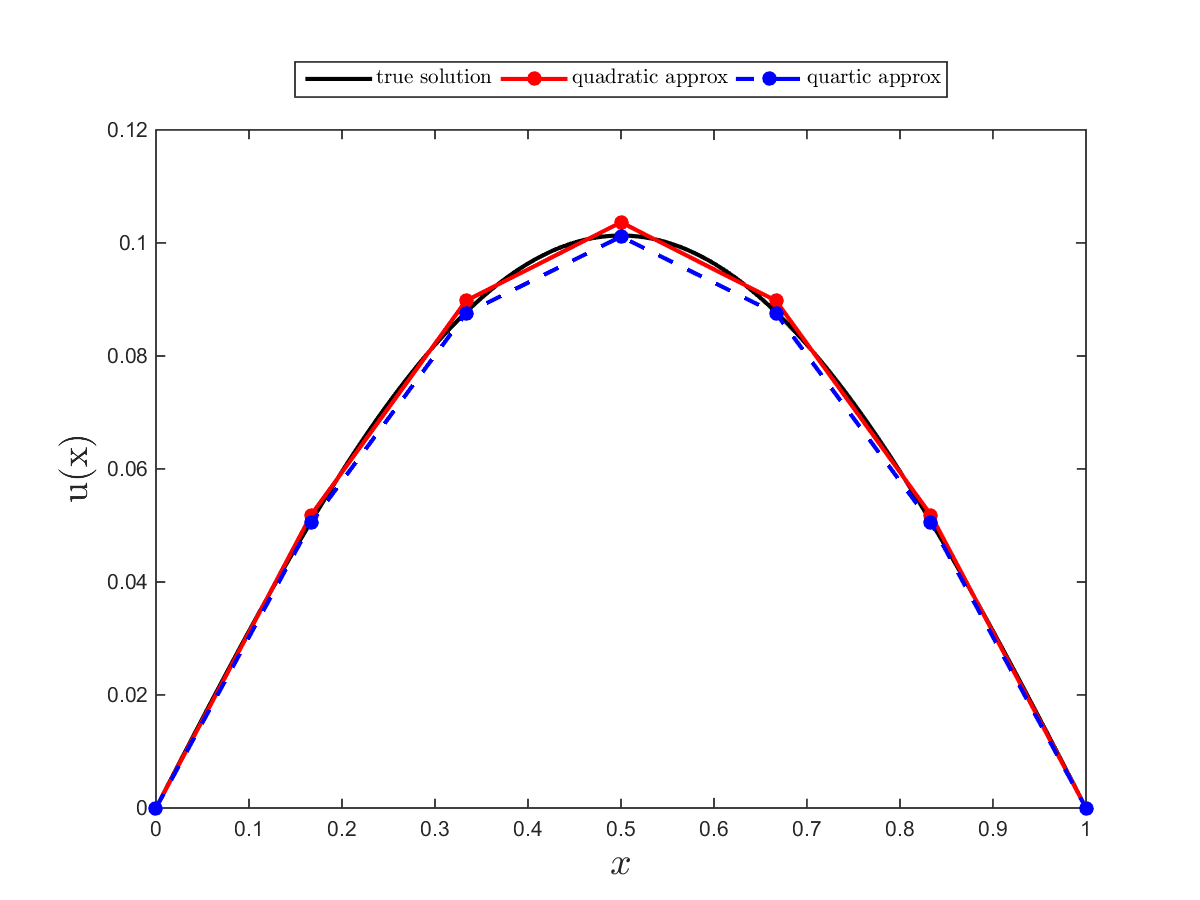
\includegraphics[scale=0.52]{quartic_approx.png}
			\caption{Quadratic and Quartic approximation}
		\end{center}
	\end{figure}
	\begin{figure}[htp]
		\begin{center}
			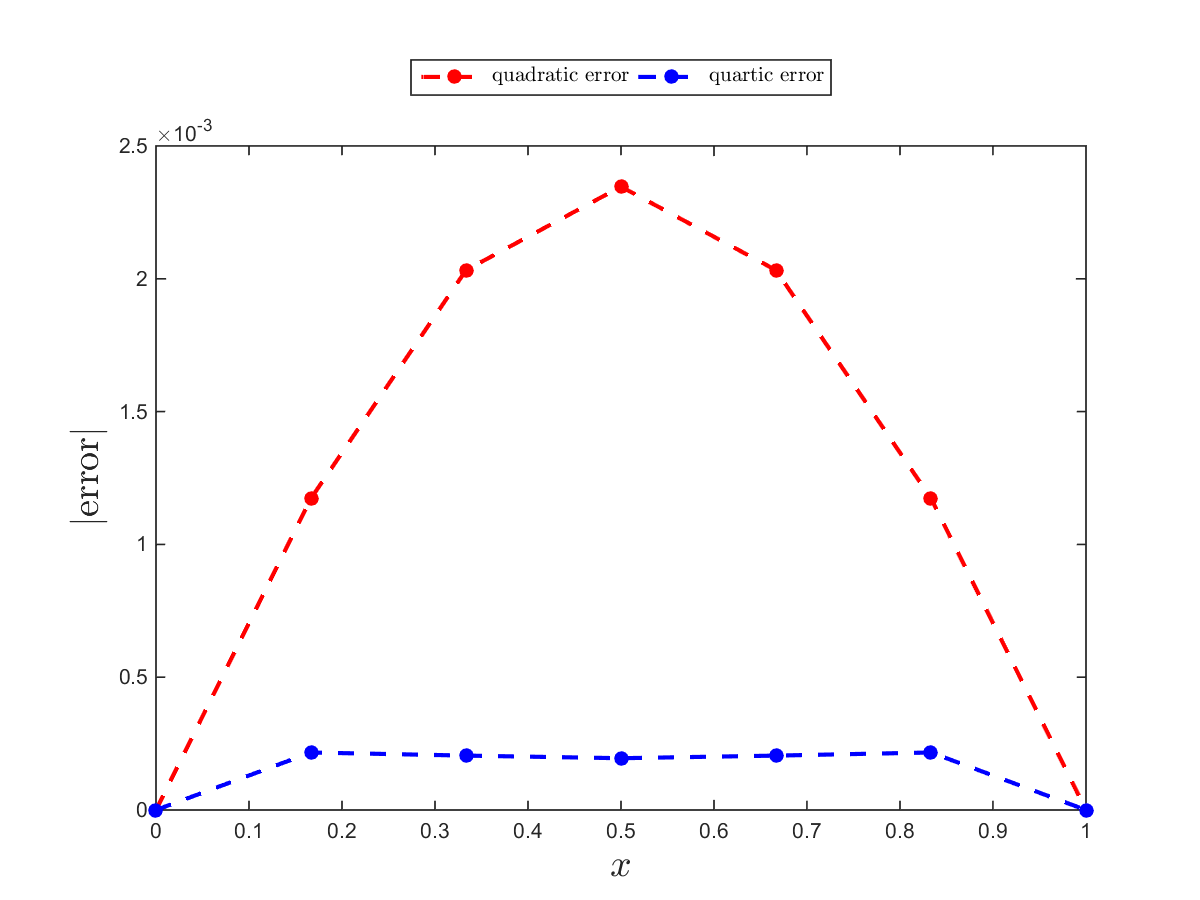
\includegraphics[scale=0.52]{quartic_error.png}
			\caption{Quadratic and Quartic error}
		\end{center}
	\end{figure}
	%\pagebreak
	
	\label{1f}
	\item Edit the code \texttt{fd\_bvp\_conv} to incorporate new approximation and produce a \texttt{loglog} plot showing:\\
	\hspace*{5cm} $ \max\limits_{0 \leq j \leq n}|u(x_j) - u_j|$ \\
	for the approximations with $n = 16, 32, 64, ..., 512$ for both the quadratic approximation and the new quartic approximation.\\
	\begin{lstlisting}
% computed constants from 1b and 1c
A = -1/12; B = 4/3; C = -5/2;
D = 11/12; E = -5/3; F = 1/2; G = 1/3; H = -1/12;
g = @(x) sin(pi*x);
true_u  = @(x) (1/pi^2)*sin(pi*x);
xx = linspace(0,1,500);
nvec = 2.^[4:9];
err2 = zeros(length(nvec),1);
err4 = zeros(length(nvec),1);

for j=1:length(nvec)
	n = nvec(j);
	h = 1/n;
	x = [0:n]'*h;
	f = -g(x(2:n));
	% Quadratic approximation
	A2 = (-2*eye(n-1)+diag(ones(n-2,1),1)+diag(ones(n-2,1),-1))/h^2;
	u2 = A2\f;
	u2 = [0;u2;0];            % add in Dirichlet values, u(0)=u(1)=0
	err2(j) = max(abs(true_u(x)-u2));
	% Quartic approximation
	A41 = [-E, -F,-G,H, zeros(1,n-5)]/h^2;
	A42n2 = (-A*diag(ones(n-2,1),-1) - B*eye(n-1) -C*diag(ones(n-2,1),1) ...
			 - B*diag(ones(n-3,1),2) -A*diag(ones(n-4,1),3))/h^2;
	A42n2(n-1,:) = []; 	A42n2(n-2,:) = [];
	A4n = [zeros(1,n-5), -H, -G,-F,-E]/h^2;
	A4 = [A41;A42n2;A4n];
	u4 = A4\f;
	u4 = [0;u4;0];
	err4(j) = max(abs(true_u(x)-u4));
end

figure(1), clf
loglog(nvec, err2,'r.-','linewidth',2,'markersize',24)
hold on;
loglog(nvec, nvec.^(-2),'r--','linewidth',2,'markersize',24)
xlabel('$n$','fontsize',18,'interpreter','latex')
ylabel('max error at grid points','fontsize',18,'interpreter','latex')
leg = legend('quadratic error','$O(h^2)$','location',...
				'northoutside','orientation','horizontal');
set(leg,'interpreter','latex','fontsize',16)
print('quadratic_approx_error_Oh','-dpng');

figure(2), clf
loglog(nvec, err4,'r.-','linewidth',2,'markersize',24)
hold on
loglog(nvec, nvec.^(-2),'b--','linewidth',2,'markersize',24)
xlabel('$n$','fontsize',18,'interpreter','latex')
ylabel('max error at grid points','fontsize',18,'interpreter','latex')
leg = legend('quartic error','$O(h^2)$','location',...
				'northoutside','orientation','horizontal');
set(leg,'interpreter','latex','fontsize',16)
print('quartic_approx_error_Oh','-dpng');
	\end{lstlisting}
	\begin{figure}[htp]
		\begin{center}
			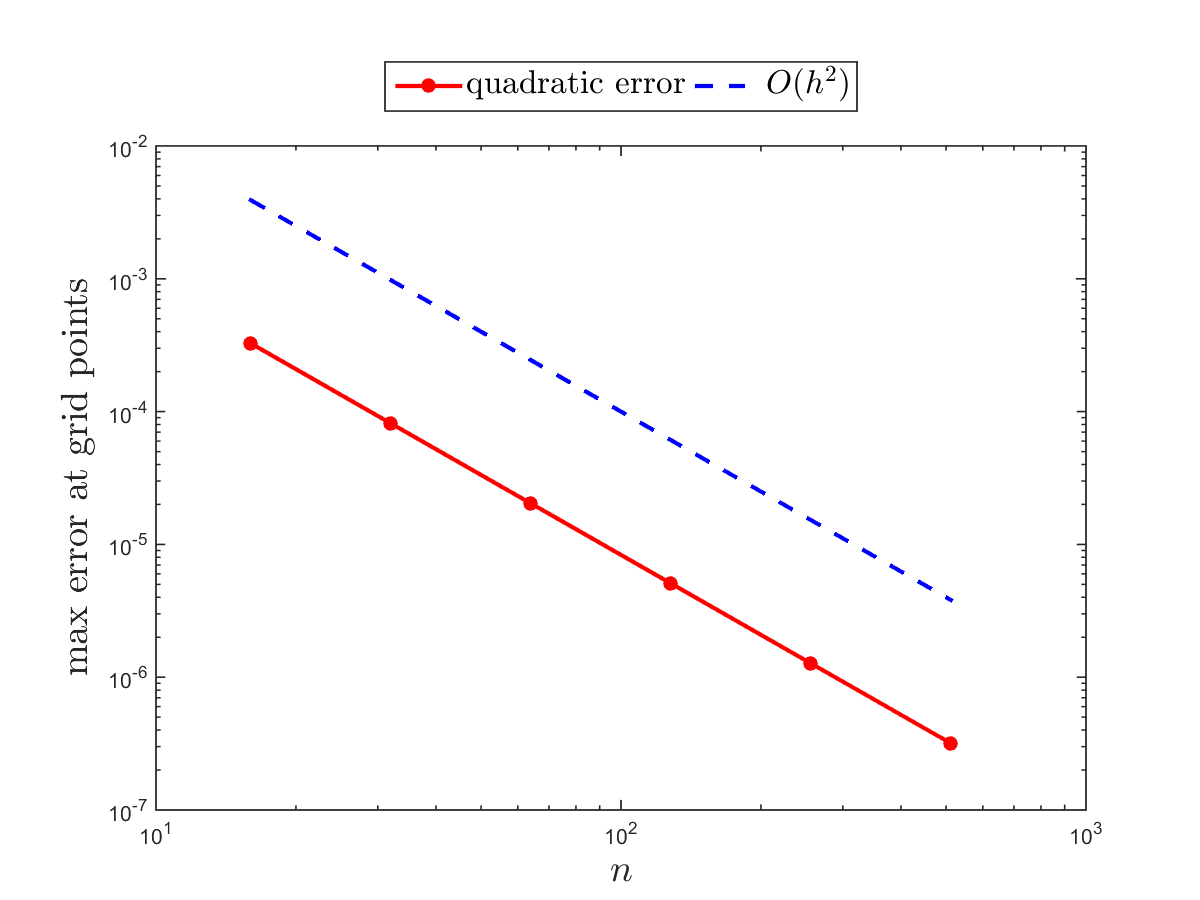
\includegraphics[scale=0.65]{quadratic_approx_error_Oh.png}
			\caption{Quadratic approximation and O(h) error}
		\end{center}
	\end{figure}
	\begin{figure}[htp]
		\begin{center}
			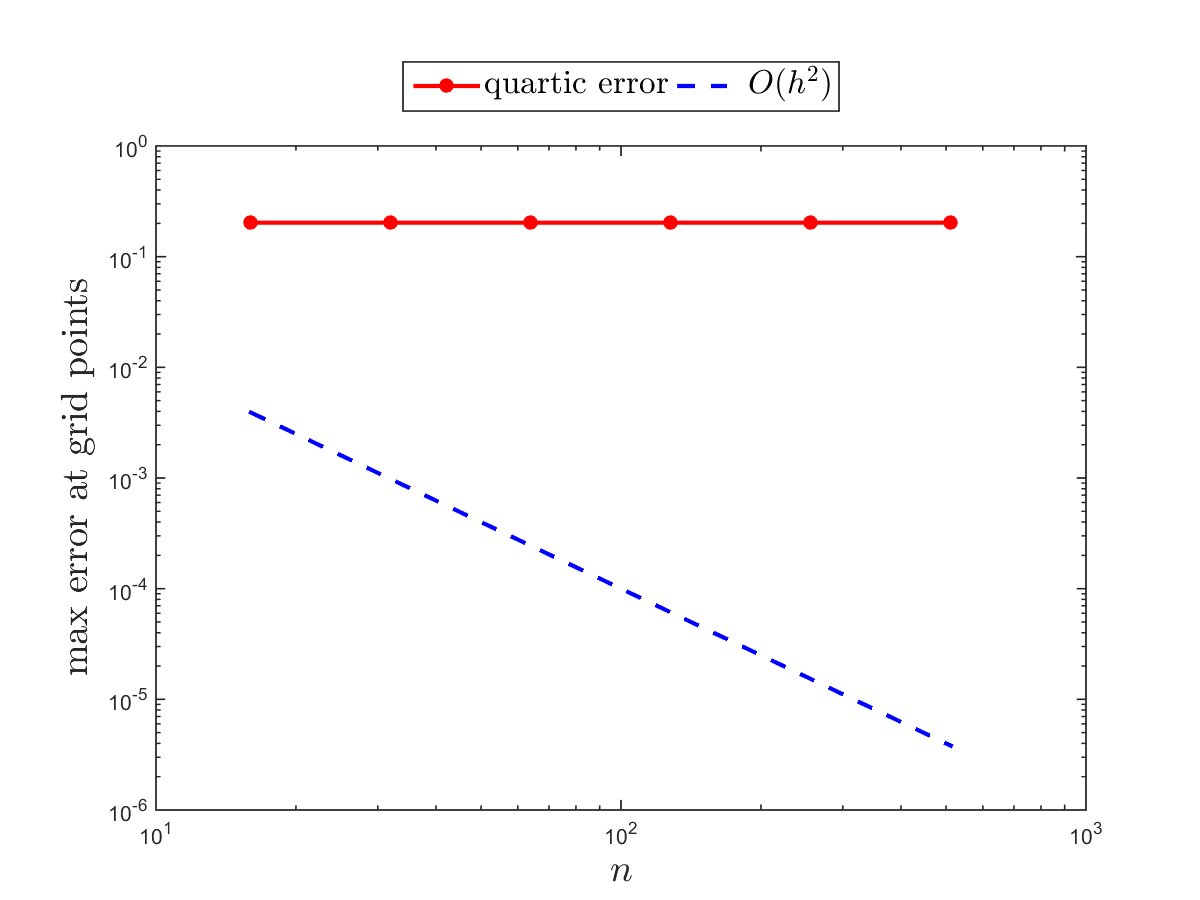
\includegraphics[scale=0.65]{quartic_approx_error_Oh.png}
			\caption{Quartic approximation and O(h) error}
		\end{center}
	\end{figure}
	
	- The quadratic approximation yielded $O(h^2)$ accuracy. What accuracy does the quartic approximation produce? Add a dashed line to your plot reflect the appropriate convergence rate of the quartic approximation.\\
	
	\label{1g}
	\item (optional) Suppose we change the left boundary condition$u'(0) = 0$. Discuss how you would implement this boundary condition while maintaining the accuracy of the approximation. Test your method out on the equation $-u"(x) = cos(\pi x/2)$ with exact solution  $u(x) = (4/\pi^2) cos(\pi x/2)$\\
	
	
	
	
\end{enumerate}

\label{Problem 2}
\large\textbf{Problem 2.} Solve these three problems from Gautschi's text:
\begin{enumerate}
	\label{2a}
	\item Consider the piecewise cubic function:\\
	\hspace*{5cm} $S(x) = \begin{cases} p(x) & \quad x \in [0,1] \\ (2-x)^3 & \quad x \in [1,2] \end{cases}$\\
	Find the cubic $p$ such that $S(0) = 0$ and $S$ is a cubic spline for the knots $x_0 = 0, x_1 = 1, x_2 = 2$. \\
	\textbf{\textit{Assume}} $p(x)$ has form: \hspace{1cm} $p(x) = a_0 + a_1x + a_2x^2 + a_3x^3$\\
	So: \hspace{4.9cm} $p'(x) = a_1 + 2a_2x + 3a_3x^2$\\
	\hspace*{5.65cm} $p"(x) = 2a_2 + 6a_3x$\\
	We have: $S(0) =0 \Rightarrow S(0) = p(0) = a_0 + a_1.0 + a_2.0^2 + a_3.0^3 = a_0 \Leftrightarrow a_0 = 0$ \\
	\hspace*{1cm} $S(1) = p(1) = 0 + a_1.1 + a_2.1^2 + a_3.1^3 = (2-1)^3 \\
	\hspace*{3.2cm} \Leftrightarrow a_1 + a_2 + a_3 = 1$ \hspace{5cm} (1) \\
	\hspace*{1cm} $S'(1) = p'(1) = a_1 + 2a_2.1 + 3a_3.1^2 = \left.[(2-x)^3]' \right|_{x=1} \\
	\hspace*{3.4cm} \Leftrightarrow a_1 + 2a_2 + 3a_3 = \left. -3(2-x)^2\right|_{x=1}\\
	\hspace*{3.4cm} \Leftrightarrow a_1 + 2a_2 + 3a_3 = -3$ \hspace{4.1cm} (2) \\
	\hspace*{1cm} $S"(1) = p"(1) = 2a_2 + 6a_3.1 = \left.[(2-x)^3]"\right|_{x=1} \\
	\hspace*{3.6cm} \Leftrightarrow 2a_2 + 6a_3 = \left. 6(2-x)\right|_{x=1}\\
	\hspace*{3.6cm} \Leftrightarrow 2a_2 + 6a_3 = 6$ \hspace{5.2cm} (3) \\
	From (1) (2) and (3) we have: $\begin{cases} a_1 + a_2 + a_3 = 1 \\ a_1 + 2a_2 + 3a_3 = -3 \\ 2a_3 + 6a_3 = 6 \end{cases} \Leftrightarrow \begin{cases} a_1 = 12 \\ a_2 = -18 \\ a_3 = 7 \end{cases} $ \\
	The cubic $p$ is defined: \hspace{0.3cm} $p(x) = 12x - 18x^2 + 7x^3$
	
	$p"(0) = 2.(-18) + 6.7.0 = -36 \neq 0 \Rightarrow $ \textbf{\textit{The spline $S$ is not natural.}}
	
	\label{2b}	
	\item Consider the set of knots $x_0 < x_1 < ... < x_n$. One could extend the idea of splines presented in class to give functions $S$ that are polynomials of degree $d$ on each interval $[x_j,x_{j+1}]$ for $j = 0,1,...,n$ with $S \in C^p[x_0,x_n]$, i.e., $S$ and its first $p$ derivatives are all continuous on $[x_0,x_n]$. What is the dimension of the space of such functions?\\
	- The number of parameters is: $(n-1)(n+1) = n^2 -1$\\
	- The number of constraints (smoothness) is: $(n-2)(p+1) = (p+1)n - 2p - 2$\\
	$\Rightarrow$ The dimension (degree of freedom) of the space is:\\
	\hspace*{3cm} $(n^2 -1) - [(p+1)n -2p -2] = n^2 - (p+1)n +2p +1$
	%(That is how many free variables are left in $S$, after the continuity conditions are imposed? Do not count any interpolation conditions).\\
	\label{2c}
	\item Let $\Pi$ denote the linear operator that maps $f \in C[a,b]$ to its \textit{piecewise linear interpolant} at $a = x_0 < x_1 < ... < x_n = b$, (i.e., $\Pi f$ denotes the piecewise linear interpolant to $f$).\\
	%- Show that $\|\Pi g\|_{\infty} \leq \|g\|_{\infty}$ for any $g \in C[a,b]$\\
	- We have: \hspace{0.3cm} $\|g\|_{\infty} = \max\limits_{a\leq x \leq b}|g(x)|$ for any $g \in [a,b]$. So: \\
	\hspace*{1.5cm} $\|\Pi g\|_{\infty} = \max\limits_{a \leq x_i \leq b} |\Pi g(x_i)| = \max\limits_{1 \leq i \leq n}|g(x_i)| \leq \|g\|_{\infty}$ \hspace{1.5cm} \textbf{\textit{Proved!}}\\
	- With $p_*$ denote any \textit{piecewise linear polynomial for these interpolation points} $x_0, x_1, ..., x_n$. We have: \\% (e.g., $p_*$ could minimize $\|f-p\|_{\infty} $ over all piecewise linear $p$ for these interpolation points).Show that:\\
	\hspace*{1cm} $\Pi p_* = p_*$ as determination of $\Pi$ above. So that:\\
	\hspace*{1cm} $\|f- \Pi f\|_{\infty} = \|f-p_* + p_* - \Pi f\|_{\infty} \leq \|f - p_*\|_{\infty} + \|p_* - \Pi f\|_{\infty}\\
	\hspace*{7.6cm} = \|f-p_*\|_{\infty} + \|\Pi p_* - \Pi f\|_{\infty}\\
	\hspace*{7.6cm} = \|f-p_*\|_{\infty} + \|-\Pi (f-p_*)\|_{\infty}\\
	\hspace*{7.6cm} \leq \|f-p_*\|_{\infty} + \|f-p_*\|_{\infty}\\
	\hspace*{7.6cm} = 2\|f-p_*\|_{\infty}$ \hspace{1.5cm} \textbf{\textit{Proved!}} \\
\end{enumerate}

\label{Problem 3}
\large\textbf{Problem 3.} This problem continues the theme of the last problem, but now with standard degree-$n$ polynomial interpolation replacing piecewise linear interpolation.\\
Let $\Pi_n$ denote the linear operator that maps $f \in C[a,b]$ to the polynomial $p_n$ that interpolates $f$ at the distinct points $x_0, ..., x_n, \{x_j\}_{j=0}^n \subset [a,b]$. In other words, $\Pi_nf = p_n$, where $p_n$ is the unique polynomial of degree $n$ (or less) for which $f(x_j) = p_n(x_j)$ for $ j = 0, ..., n$.
\begin{enumerate}
	\label{3a}
	\item Explain why $\Pi_n$ is a \textit{projector}: That is, for any $f \in C[a,b]$, show that $\Pi_n(\Pi_nf) = \Pi_nf$.\\
	Assume that $\Pi_np_n = q_n$, and because $\Pi_n$ is a linear operator so: \\
	- $q_n$ is a polynomial of degree $n$ \\
	- $q_n$ has $n+1$ root at the same distinct points $x_0,x_1, ...,x_n$ as $p_n$\\
	$\Rightarrow q_n = p_n$ or $\Pi_np_n = p_n \Leftrightarrow \Pi_n(\Pi_nf) = \Pi_nf \Leftrightarrow \Pi_n^2 = \Pi_n$ \\
	$\Rightarrow \Pi_n$ is a projector.\\
	
	 This infinity norm induces the \textit{operator norm}\\
	\hspace*{4cm} $ \|\Pi_n\|_{\infty} = \max\limits_{f \in C[a,b], f \not\equiv 0} \dfrac{\|\Pi_nf\|_{\infty}}{\|f\|_{\infty}} = \max\limits_{\|f\|_{\infty} =1} \|\Pi_nf\|_{\infty}$
	
	
	\label{3b}
	\item For $x_0 = a$ and $x_1 = b$, then:\\
	$ p_0(x_0) = f_0(x_0)$ as defined by Newton basic interpolation.\\
	and $\Pi_0.f_0(x_0) = p_0(x_0) \Leftrightarrow \Pi_0.f_0(a) = p_0(a) \Leftrightarrow \Pi_0 =1 \Rightarrow \|\Pi_n\|_{\infty} =1$ \\
	 $\|\Pi_0\|_{\infty} = \|\Pi_1\|_{\infty} =1$.
	for $n = 0$, $f$ is a constant line - degree of $0$ so $\max\limits_{\|f\|_{\infty} =1} \|\Pi_0f\|_{\infty} =1 \Rightarrow  \|\Pi_0\|_{\infty} = 1$\\
	\vspace{4cm}\\
	for $n = 1$, $f$ is a first order line - degree of $1$ so $\max\limits_{\|f\|_{\infty} =1} \|\Pi_1f\|_{\infty} =1 \Rightarrow  \|\Pi_1\|_{\infty} = 1$\\
	\label{3c}
	\item Recall that we can write the polynomial $p_n = \Pi_nf$ in the Lagrange form:
	\hspace*{5cm} $$\Pi_nf = \sum_{j=0}^{n}f(x_j)l_j(x)$$
	where $l_k$ denotes the $k^{th}$ Lagrange basis polynomial. We have:\\
	$$\|\Pi_nf\|_{\infty} = \max \limits_{x \in [a,b]} \left| \sum_{j=0}^{n} f(x_j)l_j(x) \right| \leq \|f\|_{\infty} \max \limits_{x \in [a,b]} \sum_{j=0}^{n}|l_j(x)|$$
	$$ \Rightarrow \max \|\Pi_nf\|_{\infty} = \|f\|_{\infty} \max \limits_{x \in [a,b]} \sum_{j=0}^{n}|l_j(x)|$$
	$$ \Rightarrow \|\Pi_n\|_{\infty} = \max\limits_{\|f\|_{\infty}=1} \|\Pi_nf\|_{\infty} = \max \limits_{\|f\|_{\infty}=1} \left( \|f\|_{\infty} \max \limits_{x \in [a,b]} \sum_{j=0}^{n}|l_j(x)| \right) = \max \limits_{x \in [a,b]} \sum_{j=0}^{n}|l_j(x)| $$
	
	\label{3d}
	\item Let $p_*$ denote any polynomial of degree $n$ (e.g., $p_*$ minimizes $\|f-p\|_{\infty}$ over all $p \in \mathbb{P}_n$). We have (replaced $p_n$ by $\Pi_n f$ because $p_n = \Pi_n f$ as mentioned above): \\
	$\|f-p_n\|_{\infty} = \|f-p_* + p_* - \Pi_n f\|_{\infty} \leq \|f-p_*\|_{\infty} + \|p_* - \Pi_n f\|_{\infty}$ \\
	But $\Pi_n$ is a projector on $\mathbb{P}_n$ so: $p_* - \Pi_n f = \Pi_n p_* - \Pi_n f = \Pi_n(p_* -f)$ \\
	$\Rightarrow \|f-p_n\|_{\infty} \leq \|f-p_*\|_{\infty} + \|\Pi_n(p_* - f)\|_{\infty} \leq \|f-p_*\|_{\infty} + \|\Pi_n\|_{\infty}\|p_* - f\|_{\infty} $ \\
	\hspace*{8.1cm} $ = \|f-p_*\|_{\infty} + \|\Pi_n\|_{\infty}\|f -p_*\|_{\infty} $ \\
	\hspace*{8.1cm} $ = (1+ \|\Pi_n\|_{\infty})\|f-p_*\|_{\infty}$.\\
	
	
	\label{3e}
	\item Computationally estimate $\|\Pi_n\|_{\infty}$ for $n = 1, ..., 20$:\\
	We have $\|\Pi_n\|_{\infty}$ is called Lebesque constant, so with:\\
	(i) uniformly spaced points $x_j = -1 + 2j/n$\\
	The asymptotic estimate: $\|\Pi_n\|_{\infty} \approx \dfrac{2^{n+1}}{e.n\log n}$ \\
	(ii) Chebyshev points $x_j = cos(j\pi /n)$ over $[-1,1]$.\\
	The asymptotic estimate: $\|\Pi_n\|_{\infty} \approx \dfrac{2}{\pi}\log(n+1) +1$\\ 
	
	We have the result for 2 above estimation:\\
	\begin{lstlisting}
	n = linspace(1,20,20);
	L = zeros(size(n));     % template for uniform spaced points x_j
	C = zeros(size(n));     % template for Chebyshev points
	for i = 1:size(n,2)
		L(1,i) = 2^(n(i)+1)/(exp(1)*n(i)*log(n(i)));
		C(1,i) = (2/pi)*log(n(i)+1) +1;
	end
	figure; plot(n,L,'r');
	xlabel('n'); ylabel('linear operator estimate Pi');
	title('LOS based on Uniform spaced points');
	print('LOS_uniform','-dpng');
	figure; plot(n,C,'b');
	xlabel('n'); ylabel('linear operator estimate Pi');
	title('LOS based on Chebyshev points');
	print('LOS_Chebyshev','-dpng');
	\end{lstlisting}
	\begin{lstlisting}
>> L
L =
1.0e+04 *
Columns 1 through 9
Inf    0.0002    0.0002    0.0002    0.0003    0.0004    0.0007     

Columns 7 through 14
0.0011  0.0019	 0.0033  0.0057	  0.0101   0.0181   0.0326

Columns 15 through 20
0.0594    0.1087    0.2002    0.3707    0.6895    1.2877

>> C
C =
Columns 1 through 11
1.4413   1.6994   1.8825   2.0246   2.1407   2.2388   2.3238 

Columns 7 through 14
2.3988   2.4659   2.5265   2.5819	2.6329   2.6801   2.7240 

Columns 15 through 20
2.7651    2.8037    2.8401    2.8745    2.9071    2.9382
	\end{lstlisting}
	\begin{figure}[htp]
		\begin{center}
			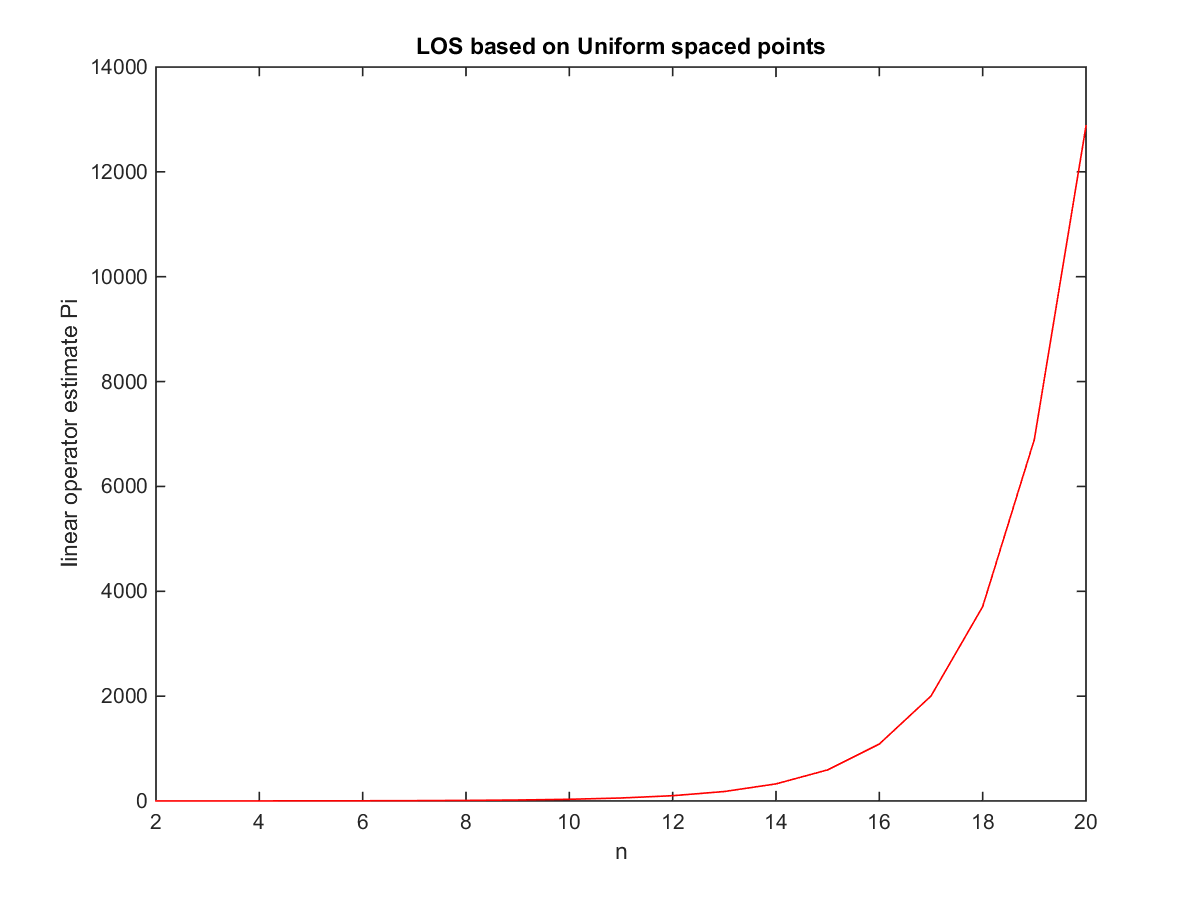
\includegraphics[scale=0.7]{LOS_uniform.png}
			\caption{Linear Operator Estimation based on uniform spaced points}
		\end{center}
	\end{figure}
	\pagebreak
	\begin{figure}[htp]
		\begin{center}
			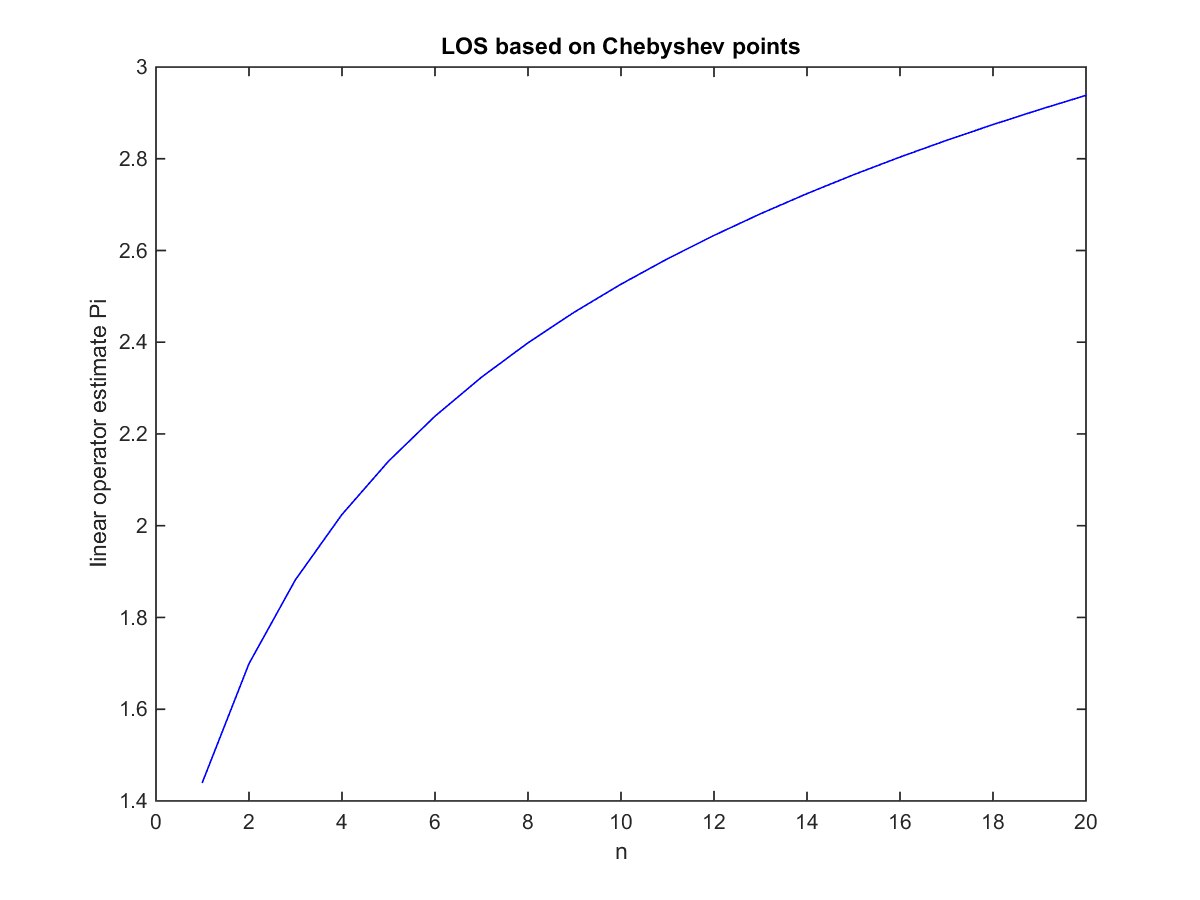
\includegraphics[scale=0.7]{LOS_Chebyshev.png}
			\caption{Linear Operator Estimation based on Chebyshev points}
		\end{center}
	\end{figure}
\end{enumerate}

\label{Problem 4}
\large\textbf{Problem 4.} \textit{Splines in font design}. The font in which this text is set was designed by Donald Knuth using his remarkable METAFONT software. To make appealing letters, the font designer establishes fixed points that guide \textit{Beriér curves}, defined via \textit{Bernstein polynomials}. These curves do not interpolate the guide points, but a similar system based on spline functions, which do interpolate, has also been proposed. Here you will try your hand at spline fond design: design a stylized 'K' character using cubic splines with natural boundary conditions. The craft would be the same if you were designing an airplane fuselage or a new sport car.\\
Consider  the following table of data. The $(f_j,g_j)$ values specify the skeleton for our 'K', as shown on the right. Our goal is to replace the straight lines by smooth curves generated from splines.\\
\begin{enumerate}
	\label{4a}
	\item Write a \texttt{MATLAB} routine: \texttt{function S = cBspline(x,x0,h)} \\
	that computes the value of a cubic B-spline at a point $x \in \mathbb{R}$, given the initial knot $x0 \in \mathbb{R}$, and uniform grid spacing $\mathtt{h}$, i.e., $x_j = x+0 + jh$.\\
	
	
	\label{4b}	
	\item Using your code from part (a), or otherwise, construct two \textit{natural} cubic splines, one, called $S_1(x)$, interpolating the $(x_j,f_j)$ values, the other, called $S_2(x)$, interpolating $(x_j,g_j)$. (Each spline should be the linear combination of $n+3=26$ B-splines. Further details are provided in the lecture notes; the variables $f_j$ and $g_j$ are defined in the $\mathtt{MATLAB}$ like $\mathtt{Kdata.m}$ on the class website).\\
	
	\label{4c}
	\item Produce a plot showing $S_1(x)$ and $S_2(x)$ for $x \in [0,23]$, along with the points $(x_j,f_j)$ and $(x_j,g_j)$ to verify that your splines interpolate the data as desired.\\
	
	\label{4d}
	\item In a separate figure, plot $(S_1(x),S_2(x))$ for $x \in [0,23]$. You should obtain a picture like the skeleton above, but with the straight lines replaced by more interesting curves. Superimpose the $(f_j,g_j)$ points to verify that your splines interpolate the data points.\\

\end{enumerate} 
	\begin{lstlisting}
n = 23;
h = 1; x0 = 0;
x = x0:n;
knots = -5:h:26;
x0indx = find(knots==x0);
pointlnd = numel(knots);
B = [];
for j = -3:n-1
B = [B, bsplinejk(x,j,3,knots,x0indx)'];
end
firstRow = [3, -6,3,zeros(1,n)];
lastRow = [zeros(1,n),3,-6,3];
B = [firstRow;B;lastRow];
Kdata;
f = [0;fj;0];
g = [0;gj;0];

cf = B\f;
cg = B\g;
xx = linspace(0,23,1000);
BB = [];
scatter(0:n,fj); legend('f_j(x_j)','S_1(x_j');
figure;
Sg = BB*cg;
plot(xx,Sg); hold on; grid on; title('S_{2}(x)');
xlabel('x_j');

for j = -3:n-1
BB = [BB, bsplinejk(x,j,3,knots,x0indx)'];
end
Sf = BB*cf;
plot(xx,Sf); hold on; grid on; title('S_{1}(x)');
xlabel('x_j');

scatter(0:n,gj); legend('g_j(x_j)','S_2(x_j');
figure;
plot(fj,gj); hold on; grid on;
legend('S_1(x_j)|S_2(x_j)','f_j(x_j)|g_j(x_j)');

	\end{lstlisting}
\end{document}